% Chapter X

\chapter{Progettazione della base di dati spaziale}
\label{ProgettazioneBasiDati}
\tikzstyle{process1} = [rectangle, minimum width=1cm, minimum height=1cm, text centered, draw=black, text width= 3cm, fill=blue!10]
\tikzstyle{process2} = [rectangle, minimum width=1cm, minimum height=1cm, text centered, draw=black,text width= 2.5cm, fill=red!30]
\tikzstyle{idEntita} = [circle, minimum width=0.01cm, minimum height=0.01cm, text centered, draw=black,text width= 0.01cm, fill=black]
\tikzstyle{attributo} = [circle, minimum width=0.01cm, minimum height=0.01cm, text centered, draw=black,text width= 0.01cm, fill=white]
\tikzstyle{arrow} = [thick,->,>=stealth]
\tikzstyle{line} = [thick,-,>=stealth]
\tikzstyle{relazione} = [diamond, minimum width=3cm, minimum height=1cm, text centered, draw=black, fill=white]

 % Chapter title
 
Avendo introdotto il metodo, esso deve poter essere verificato e validato. 
Si deve quindi poter implementare attraverso un linguaggio di programmazione lo pseudo-codice. Essendo il problema di natura geografica il campo decisionale riguardo le tecnologie che permettono di operare su questo tipo di dati è ristretto.
Nel ambito delle basi di dati, i principali DMBS supportano i dati territoriali attraverso delle componenti installabili. Questi plugin permettono l'uso di funzioni
spaziali implementate grazie alla geometria computazionale. I risultati inoltre devono poter essere consultati agevolmente per facilitare le decisioni riguardo la prevenzione del territorio. Queste esigenze si traducono nella creazione di UDF e di una basi di dati geografica che riassume i risultati ottenuti dal metodo. Sfruttando le tecnologie messe a disposizione dai sistemi GIS (Geographical Information System), sarà possibile valutare i risultati presenti nella base di dati attraverso il rendering su una mappa geografica. Tale visualizzazione contestualizza meglio i risultati rendendoli più chiari. Verrà quindi illustrata la sua progettazione attraverso le tecniche tipiche di questo ambito.
Si è progettata quindi la base di dati seguendo i seguenti passi progettuali.

\begin{figure}[H]
	\centering
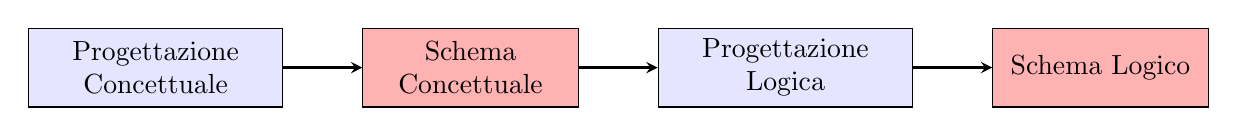
\begin{tikzpicture}[node distance=2cm]

\node (Concettuale) [process1, yshift = 1cm] {Progettazione Concettuale};
\node (SchemaConcettuale) [process2, right of= Concettuale, xshift= 2cm] {Schema Concettuale};
\node (Logica) [process1, right of= SchemaConcettuale, xshift= 2cm] {Progettazione Logica};
\node (SchemaLogico) [process2, right of= Logica, xshift= 2cm] {Schema Logico};



\draw [arrow] (Concettuale) -- (SchemaConcettuale);
\draw [arrow] (SchemaConcettuale) -- (Logica);
\draw [arrow] (Logica) -- (SchemaLogico);
\end{tikzpicture}
\caption{In figura vengono brevemente mostrati i passi concettuali nella progettazione di una base di dati. In blu vengono rappresentate le fasi concettuali. In rosso vengono rappresentati i vari schemi che si acquisiscono in output alla fine di ogni ogni fase progettuale} 
\label{fig:diagrammaER}
\end{figure}

Dalle definizioni e le notazioni introdotte nella sezione \ref{ch:notazioni} possiamo 
stabilire le entità. Esse infatti rappresentano classi di oggetti (fatti, cose, persone, ...) che hanno proprietà comuni ed esistenza autonoma ai fini dell'applicazione di interesse. Un'occorrenza di un'entità è un oggetto o istanza della classe che l'entità rappresenta.
Definiamo quindi una relazione che lega le definizioni nella sezione \ref{ch:notazioni} alle entità proposte. 
\begin{enumerate}
	\item geoarea $\leftarrow$ $GEOAREA$
	\item Zones $\leftarrow$ $\mathcal{Z}$
	\item isoipse $\leftarrow$ $\mathcal{I}$
	\item raylway\_station $\leftarrow$ $\mathcal{B}$
	\item station\_exposure $\leftarrow$ $\mathcal{EXP}$

\end{enumerate}
Tale relazione definisce le entità. Esse rappresentano concetti complessi e di rilievo che descrivono classi di oggetti con esistenza autonoma. Un'istanza di un' entità è un oggetto della classe rappresentata. Un'entità ha un nome univoco all'interno dello schema concettuale e viene rappresentata nel diagramma ER con un rettangolo con il nome dell'entità all'interno. \\
Per ogni entità vengono mostrate
\begin{enumerate}
	\item Gli attributi descritti da un pallino vuoto;
	\item L'attributo identificante descritto da un pallino nero pieno;
	\item I vincoli di partecipazione nelle relazioni, con notazione (min,max).
\end{enumerate}





\begin{figure}[H]
	\centering
	\begin{tikzpicture}[node distance=2cm]
	
	%GeoArea
	\node (GeoArea) [process1, yshift = 1cm] {GeoArea};
	\node (IdGeoArea) [idEntita, below of= GeoArea,yshift = 1cm,xshift= -1cm] {};
	\node (GeomGeoArea) [attributo, below of= GeoArea,yshift = 1cm,xshift= 1cm] {};
	
	%Zones
	\node (Zones) [process1, right of= GeoArea, xshift= 3cm] {Zones};
	\node (IdZones) [idEntita, below of= Zones,yshift = 1cm,xshift= -1cm] {};
	\node (SZK) [attributo, below of= Zones,yshift = 1cm,xshift= 1cm] {};
	\node (GeomZones) [attributo, right of = Zones,xshift = 0.5cm] {};
	
	%Isoipse
	\node (Isoipse) [process1, right of= Zones, xshift= 3cm] {Isoipse};
	\node (IdIsoipse) [idEntita, below of= Isoipse,yshift = 1cm,xshift= -1cm] {};
	\node (Elevation) [attributo, below of= Isoipse,yshift = 1cm,xshift= 1cm] {};
	\node (GeomIsoipse) [attributo, right of = Isoipse,xshift = 0.5cm] {};
	
	%RaylwayStation
	\node (RailwayStation) [process1, below of= GeoArea,yshift= -2cm] {railway\_stations};
	\node (IdRailway) [idEntita, below of= RailwayStation,yshift = 1cm,xshift= -1cm] {};
	\node (NameRailwayStation) [attributo, below of= RailwayStation,yshift = 1cm,xshift= 1cm] {};
	\node (GeomRailway) [attributo, left of = RailwayStation,xshift = -0.5cm] {};
	
	%relazione
	\node (Relazione) [relazione,right of=RailwayStation,xshift=3cm]{Ha associato};
		
	%exposure_stations	
	\node (StationExposure) [process1, right of= Relazione, xshift= 3cm] {exposure\_stations};
	\node (IdStationExposure) [idEntita, below of= StationExposure,yshift = 1cm,xshift= 0cm] {};
	\node (Exposure) [attributo, right of = StationExposure,xshift = 0.5cm] {};
		
		
	
	%GeoArea
	\draw [line] (GeoArea.south) -| node[anchor=east,yshift = -0.5cm, xshift= -0.2cm] {id} (IdGeoArea.north);
	\draw [line] (GeoArea.south) -| node[anchor=east,yshift = -0.6cm,xshift= -0.2cm] {geom}(GeomGeoArea.north);
	%Zones
	\draw [line] (Zones.south) -| node[anchor=east,yshift = -0.5cm, xshift= -0.2cm] {gid} (IdZones.north);
	\draw [line] (Zones.south) -| node[anchor=east,yshift = -0.5cm,xshift= -0.2cm] {Szk}(SZK.north);
	\draw [line] (Zones.east) -| node[anchor=south,yshift= -0.8cm] {geom}(GeomZones.west);
	%Isoipse
	\draw [line] (Isoipse.south) -| node[anchor=east,yshift = -0.5cm, xshift= -0.2cm] {gid} (IdIsoipse.north);
	\draw [line] (Isoipse.south) -| node[anchor=west,yshift = -0.5cm,xshift= 0.3cm] {Elevation}(Elevation.north);
	\draw [line] (Isoipse.east) -| node[anchor=north,yshift= 0.7cm] {geom}(GeomIsoipse.west);
	%RaylwayStation
	\draw [line] (RailwayStation.south) -| node[anchor=east,yshift = -0.5cm, xshift= -0.2cm] {gid} (IdRailway.north);
	\draw [line] (RailwayStation.south) -| node[anchor=east,yshift = -0.5cm,xshift= -0.2cm] {Name}(NameRailwayStation.north);
	\draw [line] (RailwayStation.west) -| node[anchor=north,yshift= 0.7cm] {geom}(GeomRailway.east);
	%relazione
	\draw [line] (RailwayStation.east) -| node[anchor=east,yshift = 0.3cm, xshift= -0.9cm] {(0,1)} (Relazione.west);

	\draw [line] (StationExposure.west) -| node[anchor=west,yshift = 0.3cm, xshift= 0.9cm] {(1,1)} (Relazione.east);
	%station_exposure
	\draw [line] (StationExposure.south) -| node[anchor=east,yshift = -0.5cm, xshift= -0.2cm] {gid} (IdStationExposure.north);
	\draw [line] (StationExposure.east) -| node[anchor=north,yshift= 0.7cm,xshift= 0.3cm] {exposure}(Exposure.west);
	
	
	\end{tikzpicture}
	\caption{rappresentazione diagramma Er della base di dati. sono presenti 1 associazioni ed 5 entità.} 
	\label{fig:diagrammaER}
\end{figure}

\begin{table}[H] \scriptsize
	\centering
	\renewcommand{\arraystretch}{1.2}
	\begin{tabular}{|c|c|c|c|}
		\hline
		\rowcolor[HTML]{C0C0C0} 
		Associazione           & Descrizione                                                                                                                                                                                 & Entità coinvolte                                                                                                                                                    & Attributi             \\ \hline
		\multicolumn{1}{|l|}{} & \multicolumn{1}{l|}{}                                                                                                                                                                       & \multicolumn{1}{l|}{}                                                                                                                                               & \multicolumn{1}{l|}{} \\ \hline
		ha associato           & \begin{tabular}[c]{@{}c@{}}La seguente relazione evidenzia che\\ una stazione può avere associato un valore\\ di exposure. Stessa considerazione si può fare \\ per i segmenti\end{tabular} & \begin{tabular}[c]{@{}c@{}}railway\_station\textless\textgreater      station\_exposure\\ railway\_routes\_segment\textless\textgreater segment\_exposure\end{tabular} & nessuno  \\ \hline           
	\end{tabular}
	
	\caption{descrizioni associazioni}
	\label{tab:associazioni}
\end{table}

\begin{table}[H]
	\centering
	\renewcommand{\arraystretch}{1.2} \small
	
	\begin{tabular}{|c|c|c|c|}
		\hline
		\rowcolor[HTML]{C0C0C0} 
		Entità                   & Descrizione                                                                                                                                                 & Attributi                                                           & Attributi Identificanti \\ \hline
		\multicolumn{1}{|l|}{}   & \multicolumn{1}{l|}{}                                                                                                                                       & \multicolumn{1}{l|}{}                                               & \multicolumn{1}{l|}{}   \\ \hline
		geoarea                  & \begin{tabular}[c]{@{}c@{}}Entità relativa al \\ territorio  di interesse\end{tabular}                                & \begin{tabular}[c]{@{}c@{}}id\\ geom\end{tabular}                   & id                      \\ \hline
		zones                  & \begin{tabular}[c]{@{}c@{}}Entità relativa al territorio \\ partizionato della regione abruzzo\end{tabular}                                                 & \begin{tabular}[c]{@{}c@{}}gid \\ szk\\ geom\end{tabular}           & gid                     \\ \hline
		isoipse    & \begin{tabular}[c]{@{}c@{}}Entità relativa alle isoipse contenute \\ all'interno del territorio abruzzese.\end{tabular}                                     & \begin{tabular}[c]{@{}c@{}}gid \\ elevation\\ geom\end{tabular}     & gid                     \\ \hline
		railway\_stations         & \begin{tabular}[c]{@{}c@{}}Entità relativa alle stazioni presenti \\ sul suolo della regione di interesse\end{tabular}                                      & \begin{tabular}[c]{@{}c@{}}gid \\ name\\ geom\end{tabular}          & gid                     \\ \hline
		exposure\_stations        & \begin{tabular}[c]{@{}c@{}}Entità relativa all'esposizione al rischio \\ frana da parte di una stazione\end{tabular}                                        & \begin{tabular}[c]{@{}c@{}}id\\ station\_id\\ exposure\end{tabular} & id                      \\ \hline
	
	\end{tabular}
	\caption{Descrizioni entità}
	\label{tab:entita}
\end{table}



Dallo schema Concettuale si è progettato quello logico nel seguente modo.

\begin{enumerate}
	\item geoarea(\underline{id},geom)
	\item dataset(\underline{gid},szk,geom) 
	\item isoipse\_abruzzo\_25(\underline{gid},elevation,geom)
	\item railway\_stations(\underline{gid},name,geom)
	\item exposure\_stations(\underline{id},station\_id,exposure)
	\begin{enumerate}
		\item FK: station\_id REFERENCES railway\_stations(gid)  
	\end{enumerate}
\end{enumerate}

